% ---
% school: "college"
% level: "8eme"
% section: null
% chapter: "التناظر المركزي"
% source: "Axiomaths"
% title: "تركيب : مثلث ومناظره"
% country: "Tunisie"
% year: 2026
% professor: "Axiomaths"
% difficulty: "Moyen"
% points: null
% tags: ["symetrie-centrale", "synthese", "quadrillage", "parallelogramme", "aire"]
% ---
% Exercice 7/15 de la série 8ème « التناظر المركزي » (statement + \axsol + solution). Compiler avec XeLaTeX + axiomath.sty (+ axiomaths-logo.png).
\documentclass[12pt,a4paper]{article}
\usepackage[level=8b,color=15803D]{axiomath}
\usetikzlibrary{arrows.meta}
\newcommand{\cm}{\,\mathrm{cm}}
\axsetup{title={التناظر المركزي}, corrige}

\begin{document}

\begin{corr}[title={تركيب : مثلث ومناظره}, stars=3, source={Axiomaths}]
في الشبكة المرسومة (ضلع المربع الصغير يساوي $1\cm$)، $ABC$ مثلث و $O$ نقطة.
\begin{center}
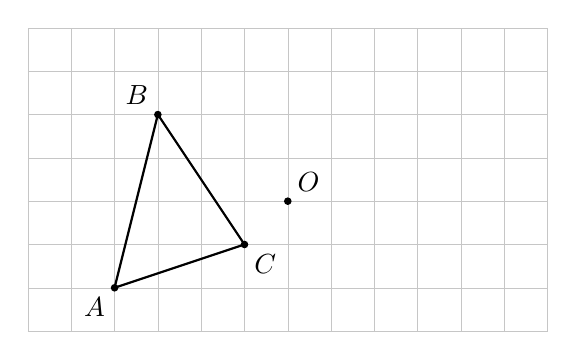
\begin{tikzpicture}[scale=0.55]
  \draw[gray!45,very thin] (0,0) grid (12,7);
  \draw[thick] (2,1)--(3,5)--(5,2)--cycle;
  \fill (6,3) circle (2.5pt) node[above right] {$O$};
  \fill (2,1) circle (2.5pt) node[below left] {$A$};
  \fill (3,5) circle (2.5pt) node[above left] {$B$};
  \fill (5,2) circle (2.5pt) node[below right] {$C$};
\end{tikzpicture}
\end{center}
\begin{enumerate}
  \item ابنِ $A'$ و $B'$ و $C'$ مناظرات $A$ و $B$ و $C$ بالنسبة إلى $O$.
  \item بين أن $ABA'B'$ متوازي أضلاع.
  \item بين أن $BCB'C'$ متوازي أضلاع.
  \item بين أن $(AB)\parallel(A'B')$ و $AB=A'B'$.
  \item احسب مساحة المثلث $ABC$ (باحتساب المربعات)، ثم استنتج مساحة $A'B'C'$.
\end{enumerate}
\axsol
\begin{enumerate}[itemsep=14pt]
  \item من $A$ إلى $O$ : 4 يمينا و 2 إلى الأعلى ؛ من $B$ إلى $O$ : 3 يمينا و 2 إلى الأسفل ؛ من $C$ إلى $O$ : وحدة يمينا ووحدة إلى الأعلى. نواصل بنفس الانتقال من $O$ فنجد $A'$ و $B'$ و $C'$.
  \begin{center}
  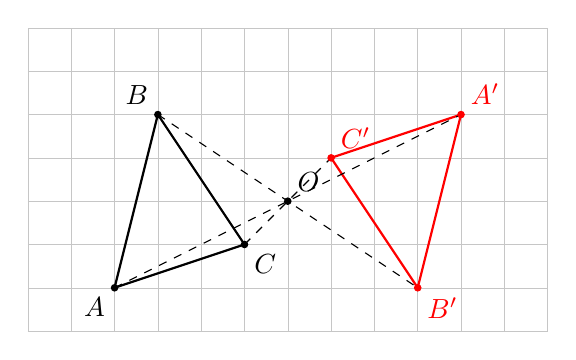
\begin{tikzpicture}[scale=0.55]
    \draw[gray!45,very thin] (0,0) grid (12,7);
    \draw[thick] (2,1)--(3,5)--(5,2)--cycle;
    \draw[thick,red] (10,5)--(9,1)--(7,4)--cycle;
    \draw[dashed] (2,1)--(10,5);
    \draw[dashed] (3,5)--(9,1);
    \draw[dashed] (5,2)--(7,4);
    \fill (6,3) circle (2.5pt) node[above right] {$O$};
    \fill (2,1) circle (2.5pt) node[below left] {$A$};
    \fill (3,5) circle (2.5pt) node[above left] {$B$};
    \fill (5,2) circle (2.5pt) node[below right] {$C$};
    \fill[red] (10,5) circle (2.5pt) node[above right] {$A'$};
    \fill[red] (9,1) circle (2.5pt) node[below right] {$B'$};
    \fill[red] (7,4) circle (2.5pt) node[above right] {$C'$};
  \end{tikzpicture}
  \end{center}
  \item\leavevmode
  \begin{prop}[رباعي قطراه لهما نفس المنتصف]
  إذا كان للقطرين نفس المنتصف فالرباعي متوازي أضلاع.
  \end{prop}
  قطرا $ABA'B'$ هما $[AA']$ و $[BB']$. $O$ منتصف $[AA']$ لأن $A'=S_O(A)$ ، و $O$ منتصف $[BB']$ لأن $B'=S_O(B)$. إذن $ABA'B'$ متوازي أضلاع.
  \item قطرا $BCB'C'$ هما $[BB']$ و $[CC']$ ، ولهما نفس المنتصف $O$. إذن $BCB'C'$ متوازي أضلاع.
  \item مناظر $[AB]$ هو $[A'B']$ ، إذن $A'B'=AB$ (حفظ الأطوال) و $(A'B')\parallel(AB)$ (مناظر مستقيم مستقيم موازٍ له). وهذا ما يؤكده الرباعي $ABA'B'$ : ضلعاه المتقابلان $[AB]$ و $[A'B']$ متوازيان.
  \item نحيط المثلث بمستطيل أبعاده $3\times4$ : مساحته $12\cm^2$. ونطرح مساحات المثلثات القائمة الثلاثة الزائدة :
  \[\dfrac{1\times4}{2}=2\ ,\qquad \dfrac{2\times3}{2}=3\ ,\qquad \dfrac{3\times1}{2}=\dfrac{3}{2}\]
  \[\mathcal{A}(ABC)=12-\left(2+3+\dfrac{3}{2}\right)=12-\dfrac{13}{2}=\dfrac{11}{2}=5{,}5\cm^2\]
  التناظر المركزي يحفظ المساحات، إذن \ib{$\mathcal{A}(A'B'C')=5{,}5\cm^2$}.
\end{enumerate}
\end{corr}

\end{document}
